\texttt{Consegne}
\begin{enumerate}
    \item Compilare e far girare il programma. Provare i controlli da keyboard. Il left mouse button aggiunge
un punto. I comandi 'f' e 'l' rimuovono il primo e l’ultimo punto dalla lista di punti, rispettivamente.
Oltre ai 64 punti, i primi punti sono rimossi.
    \item Osservare come il programma usa le OpenGL GLUT callback per catturare gli eventi click del
mouse e determinare le posizioni (x, y) relative.
    \item Provare a cambiare lo stile di punti e linee.
    \item Disegnare la curva di Bézier a partire dai punti di controllo inseriti, utilizzando l’evaluator di
OpenGL ( glMap1f(), glMapGrid1f(), glEvalMesh1()). Ricordarsi di abilitare il disegno di curve con glEnable(GL\_MAP1\_VERTEX\_3)
    \item Sostituire alle routine di OpenGL il disegno della curva mediante algoritmo di de Casteljau.
    \item Integrare nel programma in alternativa uno dei seguenti punti:
(a) disegno di una curva di Bézier mediante algoritmo ottimizzato basato sulla suddivisione adattiva.
(b) disegno interattivo di una curva di Bézier composta da tratti cubici, dove ogni tratto viene
raccordato con il successivo con continuitá C 0 , C 1 , o G 1 a seconda della scelta utente da
keyboard.
    \item Permettere la modifica della posizione dei punti di controllo tramite trascinamento con il mouse
\end{enumerate}
 \texttt{Svolgimento}
 \begin{enumerate}
     \item Nulla da dover descrivere
     \item Nulla da dover descrivere
     \item È possibile cambiare la dimensione della linea modificando il valore all'interno della funzione \textit{glLineWidth}. La dimensione dei punti invece è modificabile attraverso la chiamata a \textit{glPointSize}
     \item Il codice dell'implementazione è verificabile nel sorgente sotto la funzione \textit{drawBezierGL}, ma descrivendolo brevemente, è sufficiente utilizzare le funzioni di liberia \textit{glBegin} per iniziare a disegnare i punti, i quali verranno calcolati attraverso la funzione \textit{glEvalCoord1f}. 
     \item L'algoritmo di Casteljau è stato implementato nel seguente modo ed è verificabile nel sorgente sotto la funzione \textit{castelAlgo}:\\ 
     Per ogni valore del parametro \textit{t}, si effettuano una serie di LERP, e se i punti di controllo sono N, allora per ogni valore si effettuano $$\sum_{i=0}^{n} lerp$$, dove con lerp si intende l'interpolazione lineare, calcolata come Lerp(t,A,B)=(1-t)A+tB.\\
     A questo punto, è possibile disegnare la curva utilizzando una chiamata a \textit{glVertex3f}.
    \item E' stato scelto di integrare il punto A, utilizzare cioè la suddivisione adattiva per implementare la curva di Bezier. Anche in questo caso il sorgente è consultabile, sotto le funzioni \textit{drawBezierAdaptive} e \textit{adaptiveSubdivision}.\\
    In questo caso non viene dato il parametro \textit{t} nel quale deve essere valutata la curva, come nelle fasi precedenti, bensì un valore di tolleranza.
    La prima parte consiste nel calcolare la distanza di ogni punto dalla corda tra il primo e l'ultimo punto e, se la distanza di ogni punto intermedio è minore della tolleranza, allora la curva può essere approssimata con una linea retta.\\
    Di questa parte si occupano le prime righe del codice, in particolare \textit{pointLineDistance} che
    permette il calcolo della distanza tra ogni punto e la corda e, in caso positivo, cioè con distanza minore dalla tolleranza, si disegnano i punti con le primitive di OpenGL.\\
    In caso negativo invece, la curva viene splittata in due, aggiungendo i punti calcolati con la LERP, e il processo è iterato per le due sottocurve ricorsivamente, finchè non è possibile disegnare l'intera curva.
    \item L'implementazione è stata effettuata attraverso due callback, chiamate \textit{passive} e \textit{motion}.
    La seconda viene invocata quando avviene un drag di un punto, e si occupa di modificare le coordinate dell'elemento e di invocare la funzione di display. In realtà è invocata
    ogni volta che il mouse si muove sullo schermo, ma effettua veramente del lavoro solo quando l'utente ha cliccato un punto, grazie alla variabile \textit{isMoving}.\\
    \textit{Passive} invece ha un compito diverso, quello di identificare che l'utente stia passando sopra ad un punto di controllo o no. In caso positivo, colora il punto di controllo in cui si trova di colore rosso, distinguendolo dagli altri. Per fare ciò si calcola la distanza della posizione dal mouse da tutti i punti sullo schermo e, in caso sia minore di una certa tolleranza, marca il punto e invoca la funzione di display, che si occuperà del colore.\\
           {\centering
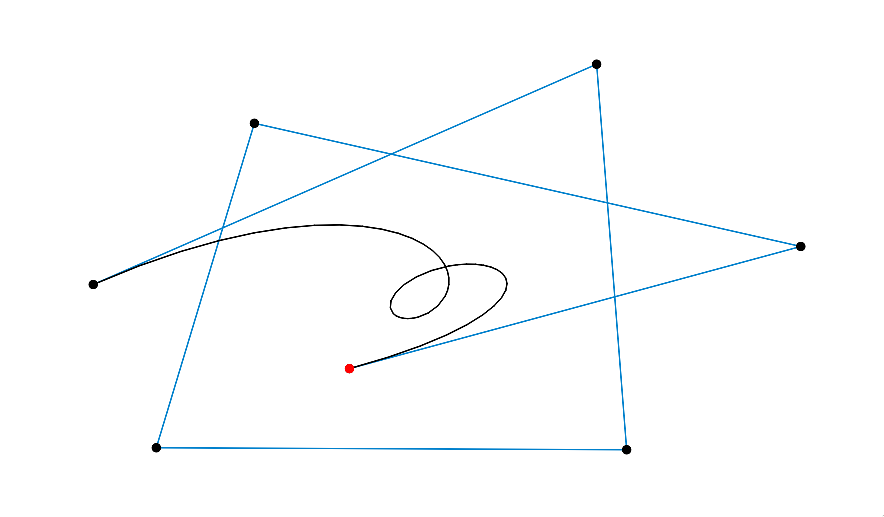
\includegraphics[width=0.6\textwidth]{bezier.png}} 
 \end{enumerate}